\documentclass[conference]{IEEEtran}
\IEEEoverridecommandlockouts

% --- Kodiranje i jezik ---
\usepackage[T1]{fontenc}
\usepackage[utf8]{inputenc}
\usepackage[serbian]{babel}   % ako pravi gresku na Overleaf-u, zameniti sa: \usepackage[english]{babel}

% --- Paketi ---
\usepackage{graphicx}
\usepackage{booktabs}
\usepackage{amsmath}
\usepackage{amssymb}
\usepackage{array}
\usepackage{url}
\usepackage{hyperref}

\graphicspath{{figures/}{../results/}}

\begin{document}

\title{Hijerarhijska klasifikacija biljnih bolesti\\
korišćenjem dubokih neuronskih mreža}

\author{\IEEEauthorblockN{Marija Tadić, E9 12/2024}
\IEEEauthorblockA{Fakultet tehničkih nauka, Univerzitet u Novom Sadu\\
Master studije --- Mašinsko učenje i veštačka inteligencija\\
Predmet: Neuronske mreže}}

\maketitle

\begin{abstract}
Rana i automatska detekcija biljnih bolesti sa fotografija listova može značajno
ubrzati dijagnostiku u poljoprivredi. U ovom radu poredimo \emph{hijerarhijski}
pristup klasifikaciji --- u kome prvi model prepoznaje vrstu biljke, a zatim
poseban model po vrsti prepoznaje bolest --- sa \emph{ravnim} pristupom koji
direktno klasifikuje svih 38 kombinacija (vrsta, bolest). Eksperimenti su
izvedeni na skupu PlantVillage (54.305 slika, 14 vrsta, 38 klasa), koji je
neuravnotežen na oba nivoa hijerarhije. Pošto skup nije balansiran, kao primarnu
metriku koristimo \emph{makro F1}, a tačnost (accuracy) prijavljujemo samo kao
sporednu. Najbolji ravni model (ResNet-50) postiže makro F1 od $0{,}9843$ na test
skupu, dok hijerarhijski pristup postiže $0{,}9741$ --- dakle hijerarhija
\emph{ne donosi poboljšanje}, već blago zaostaje. Analizom propagacije greške
pokazujemo da $21{,}1\%$ grešaka hijerarhije potiče od pogrešno prepoznate vrste,
što je nepopravljiv izvor greške koji ravni model nema. Konačno, kroz Grad-CAM
vizualizaciju i diskusiju o pristrasnosti na pozadinu (\emph{background bias})
razmatramo zašto visoke vrednosti metrika na PlantVillage skupu ne garantuju
upotrebljivost u realnim uslovima.
\end{abstract}

\begin{IEEEkeywords}
klasifikacija biljnih bolesti, hijerarhijska klasifikacija, konvolucijske
neuronske mreže, transfer learning, neuravnoteženi podaci, makro F1, PlantVillage
\end{IEEEkeywords}

\section{Uvod}
Biljne bolesti su jedan od glavnih uzročnika gubitka prinosa i kvaliteta useva.
Klasična dijagnostika zahteva iskusne stručnjake i vremenski je zahtevna, dok
automatska detekcija metodama računarskog vida može omogućiti bržu i dostupniju
dijagnostiku, uključujući i terensko skeniranje na uređajima ograničenih resursa.

Cilj ovog rada je razvoj i evaluacija sistema za automatsku klasifikaciju biljnih
bolesti sa fotografija listova primenom dubokih konvolucijskih neuronskih mreža.
Posebno ispitujemo \emph{hijerarhijski} pristup: kompleksan problem sa 38 klasa
deli se na dva jednostavnija zadatka --- prepoznavanje vrste biljke (nivo 1) i,
unutar prepoznate vrste, prepoznavanje tipa bolesti (nivo 2). Pretpostavka je da
ovakva dekompozicija može poboljšati interpretabilnost i, eventualno,
performanse. Da bismo proverili tu pretpostavku, kao referentnu tačku
implementiramo \emph{ravni} klasifikator sa 38 klasa, te eksplicitno poredimo dva
pristupa.

Glavni doprinosi rada su: (1) implementacija i poređenje ravnog i hijerarhijskog
pristupa pod istim uslovima; (2) evaluacija prilagođena neuravnoteženom skupu, sa
makro F1 kao primarnom metrikom; (3) kvantifikacija \emph{propagacije greške} u
hijerarhiji; i (4) kritička diskusija o pristrasnosti na pozadinu i o tome zašto
visoke metrike na PlantVillage skupu treba tumačiti sa oprezom.

\section{Srodni radovi}
Mohanty i saradnici~\cite{mohanty2016} prvi su primenili duboke mreže (AlexNet,
GoogLeNet) na PlantVillage skup i postigli tačnost preko $99\%$, ali su uočili da
performanse naglo opadaju na slikama snimljenim van kontrolisanih uslova.
Ferentinos~\cite{ferentinos2018} proširuje ovaj pravac na veći broj arhitektura i
klasa, potvrđujući visoku tačnost na laboratorijskim slikama. Too i
saradnici~\cite{too2019} porede fino podešavanje (\emph{fine-tuning}) više
arhitektura, dok Mohameth i saradnici~\cite{mohameth2020} analiziraju ekstrakciju
obeležja naspram finog podešavanja. Noyan~\cite{noyan2022} kritički ukazuje na
\emph{pristrasnost na pozadinu}: zbog gotovo uniformne pozadine po klasi, modeli
mogu naučiti pozadinu umesto same lezije, što objašnjava slabu generalizaciju na
terenske slike. Naš rad se nadovezuje na ovu kritiku: pored poređenja arhitektura
i pristupa, eksplicitno merimo propagaciju greške i koristimo Grad-CAM~\cite{gradcam2017}
za vizuelnu analizu na šta model obraća pažnju.

\section{Metodologija}

\subsection{Skup podataka i podela}
Korišćen je PlantVillage skup (\emph{color} verzija), sa $54.305$ RGB slika
listova razvrstanih u 38 klasa koje predstavljaju kombinaciju vrste biljke i
bolesti, raspoređenih u 14 biljnih vrsta. Skup je \emph{neuravnotežen} na oba
nivoa: odnos najveće i najmanje klase iznosi približno $48{,}9{:}1$ na nivou
vrste i $36{,}2{:}1$ na nivou bolesti. Dodatno, 5 od 14 vrsta ima samo jednu
klasu (zdravo stanje), pa su za njih klasifikatori bolesti trivijalni.

Skup je podeljen na trening, validacioni i test deo u odnosu $70{:}15{:}15$
primenom \emph{stratifikovane} podele (uz fiksni seed $42$), čime se očuvava
raspodela klasa u svakom delu. Podela je perzistirana u CSV datotekama i nikada
se ne regeneriše, čime se obezbeđuje reproducibilnost. Rezultujuće veličine su
$38.013$ (trening), $8.146$ (validacija) i $8.146$ (test) slika.

\subsection{Pretprocesiranje i augmentacija}
Sve slike su skalirane na $224\times224$ piksela i normalizovane statistikom
ImageNet skupa. Nad trening skupom primenjena je \emph{agresivna} augmentacija
(slučajno isecanje i skaliranje, horizontalno i vertikalno preslikavanje,
rotacije, afine i perspektivne transformacije, promene boje/osvetljenja, te
slučajno brisanje regiona --- \emph{random erasing}). Agresivna augmentacija je
namerna mera protiv pristrasnosti na pozadinu: cilj je primorati model da se
oslanja na teksturu lista i lezije, a ne na uniformnu pozadinu. Nad
validacionim i test skupom \emph{ne} primenjuje se augmentacija.

\subsection{Modeli}
Implementirana su tri tipa modela:
\begin{itemize}
  \item \textbf{Bazni CNN} treniran od nule (4 konvolucijska bloka sa batch
  normalizacijom, globalnim pooling-om i dropout-om, $\approx1{,}3$M parametara)
  --- služi kao referentna tačka ``od nule''.
  \item \textbf{ResNet-50} sa ImageNet pretreniranim težinama (transfer
  learning), uz fino podešavanje poslednje dve etape i klasifikacionog sloja.
  \item \textbf{EfficientNet-B0} (podržan u implementaciji kao lakša
  alternativa); glavni izveštaji odnose se na ResNet-50 kao reprezentativan
  transfer model.
\end{itemize}
Hijerarhijski sistem se sastoji od jednog modela za vrstu (14 klasa) i rečnika
modela za bolest --- po jednog za svaku od 9 netrivijalnih vrsta; pet vrsta sa
jednom klasom rutira se direktno. U fazi predikcije, izlaz modela za vrstu bira
odgovarajući model za bolest.

\subsection{Treniranje i tretiranje neuravnoteženosti}
Modeli su trenirani optimizatorom AdamW (varijanta Adama sa razdvojenom
regularizacijom težina), uz kosinusni raspored stope učenja, ranо zaustavljanje
(\emph{early stopping}) i čuvanje najboljeg modela prema \emph{validacionom makro
F1} (a ne prema gubitku). Za tretiranje neuravnoteženosti koristi se
\emph{ponderisana} unakrsna entropija (\emph{weighted cross-entropy}), sa
težinama izvedenim iz frekvencija klasa u trening skupu; implementacija takođe
podržava \emph{focal} gubitak~\cite{focal2017} i ponderisano uzorkovanje.
Treniranje je izvedeno na Kaggle GPU (Tesla T4), a razvoj koda lokalno.

\subsection{Evaluacija}
Pošto skup nije balansiran, tačnost (accuracy) nije reprezentativna metrika i
prijavljuje se samo kao sporedna. Primarne metrike su: \textbf{makro F1} (tretira
sve klase jednako), \emph{ponderisani} F1, \emph{balansirana tačnost}, te
precision/recall po klasi i matrica konfuzije. Za hijerarhiju se računaju
\emph{end-to-end} metrike na finalnoj (vrsta, bolest) predikciji, kao i
\emph{propagacija greške} --- udeo grešaka koje potiču od pogrešno prepoznate
vrste.

\section{Rezultati}

\subsection{Ravni modeli}
Na validacionom skupu, bazni CNN (od nule) postiže makro F1 od $0{,}9826$, a
ResNet-50 (transfer) $0{,}9882$. Pretreniranje na ImageNet skupu donosi samo
$\approx0{,}5$ procentnih poena, što ukazuje da je zadatak na ovom skupu gotovo
zasićen i da ga čak i jednostavna mreža od nule rešava skoro savršeno.
Slika~\ref{fig:curves} prikazuje krive učenja.

\begin{figure}[t]
  \centering
  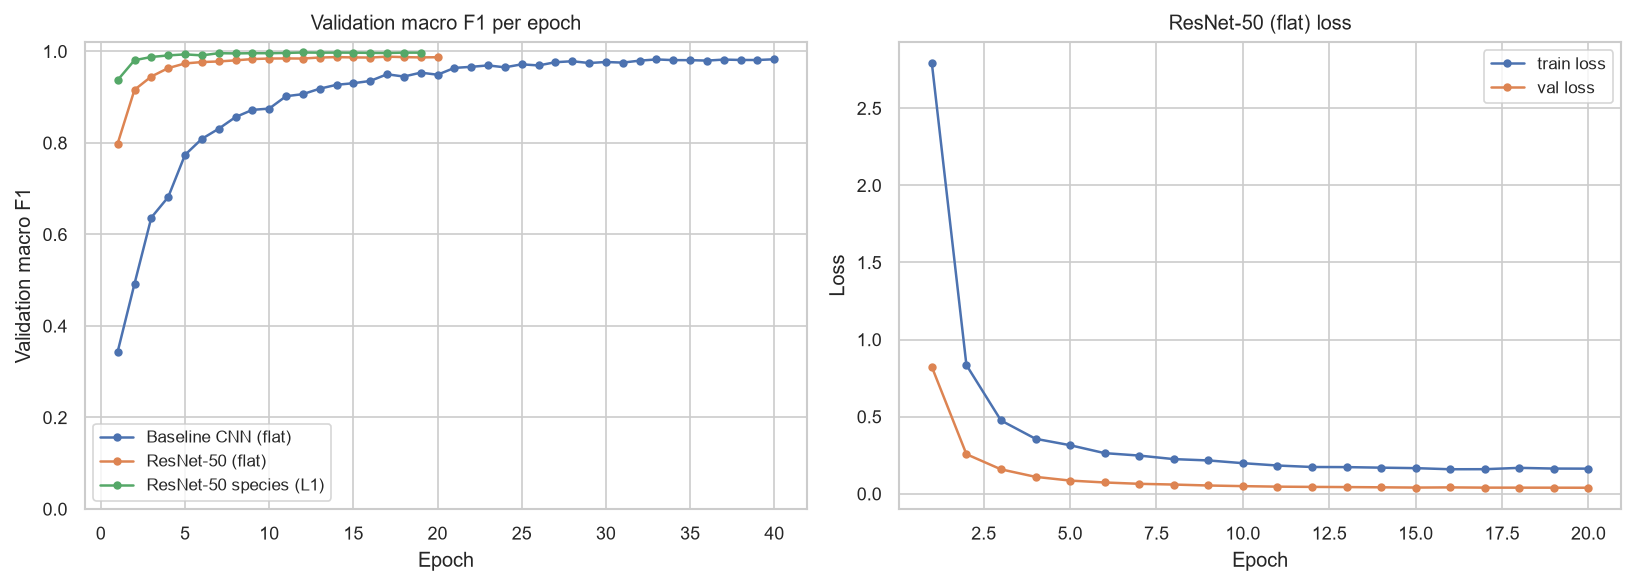
\includegraphics[width=\columnwidth]{training_curves.png}
  \caption{Validacioni makro F1 po epohama (levo) i gubitak za ResNet-50 (desno).}
  \label{fig:curves}
\end{figure}

\subsection{Hijerarhija: nivoi}
Model za vrstu (nivo 1) postiže makro F1 od $0{,}9974$ na validaciji ---
prepoznavanje vrste je gotovo savršeno, što sugeriše mali doprinos propagacije
greške sa prvog nivoa. Klasifikatori bolesti (nivo 2) variraju po vrsti
(Tabela~\ref{tab:disease}, Slika~\ref{fig:heads}): od savršenih kod binarnih
vrsta do najtežih --- krompir ($0{,}9047$) i kukuruz ($0{,}9467$).

\begin{table}[t]
  \caption{Makro F1 klasifikatora bolesti po vrsti (validacija).}
  \label{tab:disease}
  \centering
  \begin{tabular}{lcc}
    \toprule
    Vrsta & Broj bolesti & Makro F1 \\
    \midrule
    Cherry      & 2  & 1{,}0000 \\
    Strawberry  & 2  & 1{,}0000 \\
    Peach       & 2  & 0{,}9947 \\
    Pepper bell & 2  & 0{,}9944 \\
    Grape       & 4  & 0{,}9935 \\
    Apple       & 4  & 0{,}9865 \\
    Tomato      & 10 & 0{,}9764 \\
    Corn        & 4  & 0{,}9467 \\
    Potato      & 3  & 0{,}9047 \\
    \bottomrule
  \end{tabular}
\end{table}

\begin{figure}[t]
  \centering
  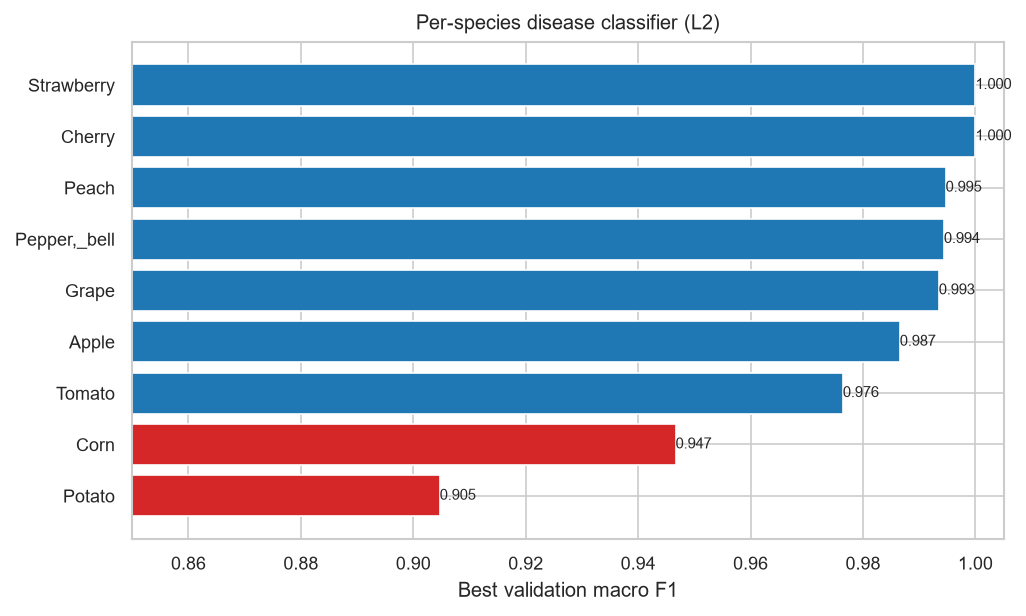
\includegraphics[width=\columnwidth]{disease_heads_macro_f1.png}
  \caption{Makro F1 klasifikatora bolesti po vrsti; crvenom su označene
  najslabije (Potato, Corn).}
  \label{fig:heads}
\end{figure}

\subsection{Ravni pristup naspram hijerarhije}
Tabela~\ref{tab:main} i Slika~\ref{fig:flatvshier} prikazuju glavni rezultat na
\emph{test} skupu. Ravni ResNet-50 postiže makro F1 od $0{,}9843$, dok
hijerarhija postiže $0{,}9741$ --- razlika je $-0{,}0102$ u korist ravnog
pristupa. Isti trend važi i za ostale metrike.

\begin{table}[t]
  \caption{Ravni naspram hijerarhijskog pristupa (test skup). Makro F1 je
  primarna metrika; tačnost je sporedna.}
  \label{tab:main}
  \centering
  \begin{tabular}{lccc}
    \toprule
    Metrika & Ravni & Hijerarhija & $\Delta$ \\
    \midrule
    Makro F1            & \textbf{0{,}9843} & 0{,}9741 & $-0{,}0102$ \\
    Ponderisani F1      & 0{,}9868 & 0{,}9821 & $-0{,}0047$ \\
    Balansirana tačnost & 0{,}9859 & 0{,}9813 & $-0{,}0046$ \\
    Tačnost (sporedno)  & 0{,}9867 & 0{,}9820 & $-0{,}0047$ \\
    \bottomrule
  \end{tabular}
\end{table}

\begin{figure}[t]
  \centering
  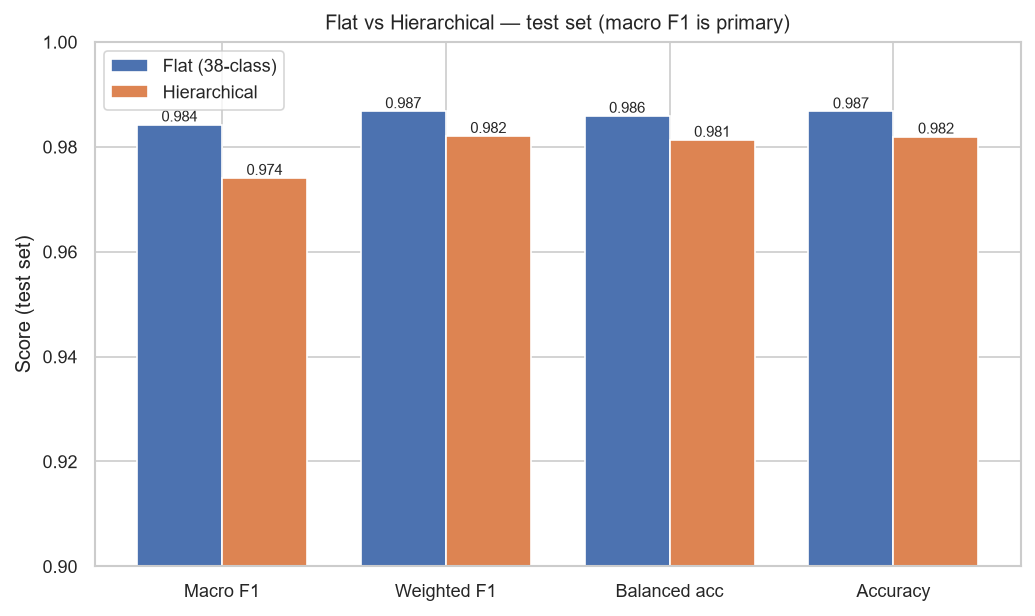
\includegraphics[width=\columnwidth]{flat_vs_hierarchical.png}
  \caption{Ravni naspram hijerarhijskog pristupa na test skupu.}
  \label{fig:flatvshier}
\end{figure}

\subsection{Propagacija greške}
Na test skupu, model za vrstu je tačan u $99{,}62\%$ slučajeva, a klasifikacija
bolesti uz tačnu vrstu postiže makro F1 od $0{,}9815$. Od ukupno $147$ end-to-end
grešaka hijerarhije, $31$ potiče od pogrešne vrste (nepopravljivo), a $116$ od
pogrešne bolesti pri tačnoj vrsti. Dakle, $21{,}1\%$ svih grešaka uzrokovano je
prvim nivoom (Slika~\ref{fig:errprop}). Ravni model nema ovaj kaskadni izvor
greške, što objašnjava njegovu blagu prednost.

\begin{figure}[t]
  \centering
  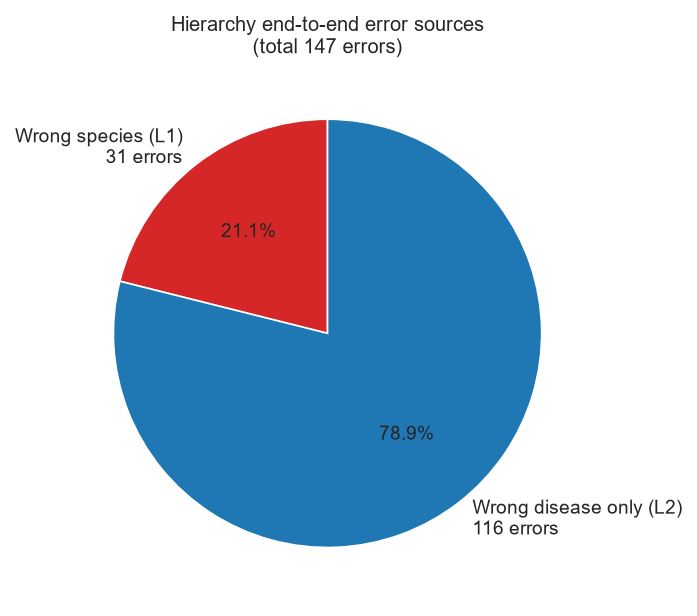
\includegraphics[width=0.85\columnwidth]{error_propagation.png}
  \caption{Izvori end-to-end grešaka hijerarhije.}
  \label{fig:errprop}
\end{figure}

\subsection{Analiza grešaka}
Matrica konfuzije ravnog modela (Slika~\ref{fig:cm}) pokazuje izraženu dijagonalu
uz greške koncentrisane među bolestima paradajza i kukuruza. Najslabije klase po
F1 su Tomato Early blight ($0{,}89$), Corn Cercospora/Gray leaf spot ($0{,}91$) i
Tomato Late blight ($0{,}94$). Najčešća zabuna je između dve gljivične bolesti
kukuruza; uočena je i \emph{međuvrsna} zabuna --- Potato Late blight predviđen kao
Tomato Late blight --- što odgovara činjenici da je reč o istoj bolesti na srodnim
biljkama.

\begin{figure}[t]
  \centering
  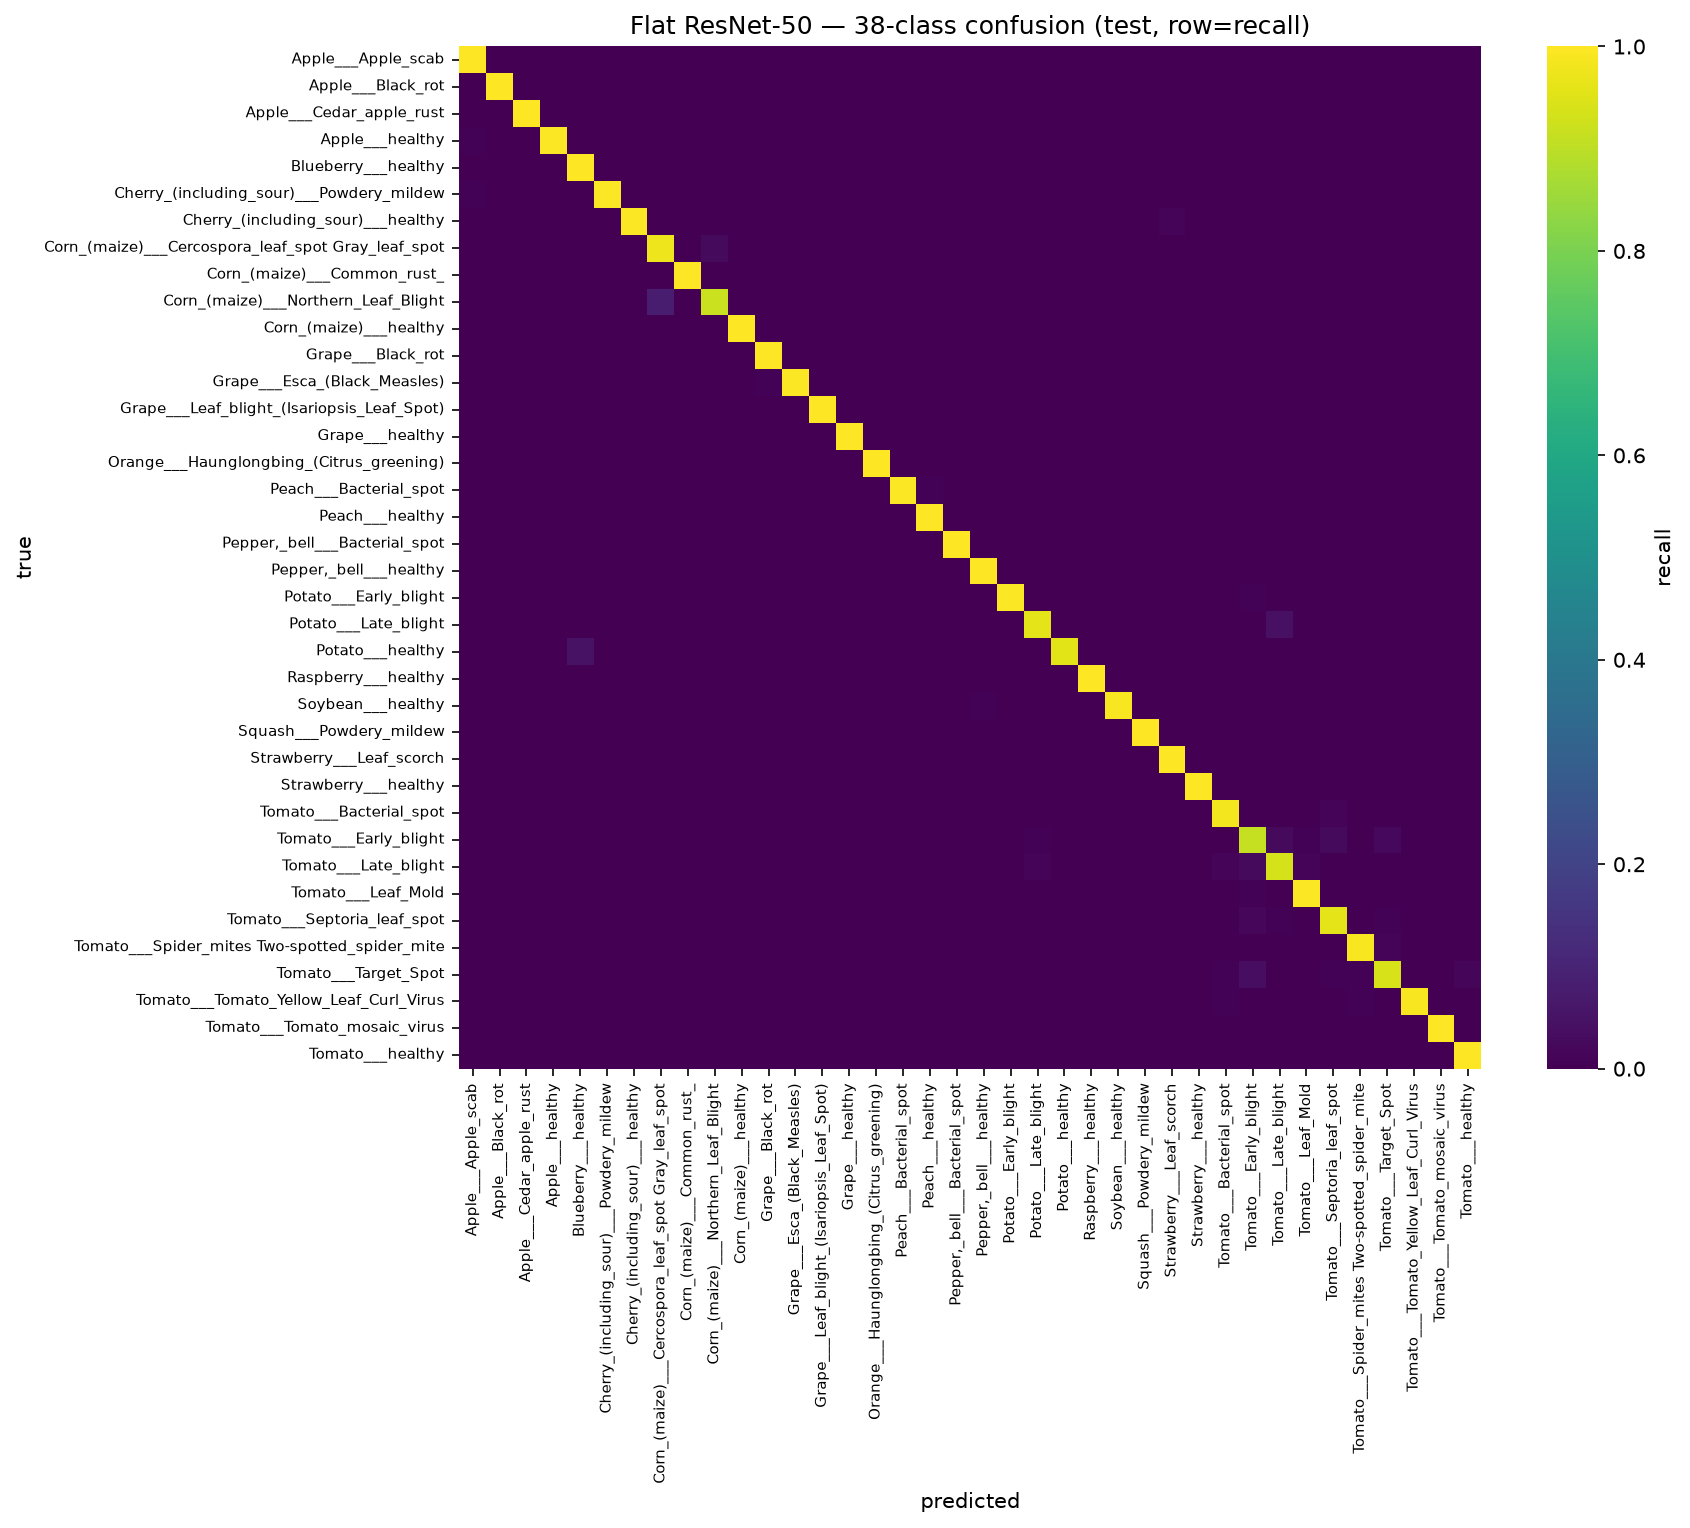
\includegraphics[width=\columnwidth]{confusion_flat.png}
  \caption{Matrica konfuzije ravnog ResNet-50 modela (test, normalizovano po
  redu = recall po klasi).}
  \label{fig:cm}
\end{figure}

\section{Diskusija}

\subsection{Zašto hijerarhija ne pomaže}
Iako intuitivno deluje da dekompozicija problema treba da pomogne, na ovom skupu
hijerarhija blago zaostaje. Razlog je dvojak: (1) ravni model već postiže
$\approx0{,}98$, pa je prostor za poboljšanje mali; i (2) hijerarhija uvodi
dodatnu tačku otkaza --- greške na nivou vrste su nepopravljive i čine petinu svih
grešaka. Ravni model zajednički modeluje (vrsta, bolest) i izbegava kaskadu.
Ovo je validan rezultat: hijerarhijski pristup nije uvek opravdan.

\subsection{Visoke metrike i pristrasnost na pozadinu}
Vrednosti metrika na PlantVillage skupu su veoma visoke za sve modele, što je u
skladu sa literaturom~\cite{mohanty2016,ferentinos2018}. Međutim, ove vrednosti
ne treba tumačiti kao meru upotrebljivosti u praksi. PlantVillage slike su
snimane u kontrolisanim uslovima, sa gotovo uniformnom pozadinom po klasi, pa
model može naučiti pozadinu kao prečicu~\cite{noyan2022}. Grad-CAM analiza
(Slika~\ref{fig:gradcam}) pokazuje da model uglavnom obraća pažnju na tkivo
lista, ali difuzno --- ne precizno na leziju. Pošto list popunjava gotovo ceo
kadar, pristrasnost na pozadinu se na ovim slikama teško direktno uočava; glavni
rizik ostaje slaba generalizacija na terenske slike sa drugačijom pozadinom.

\begin{figure}[t]
  \centering
  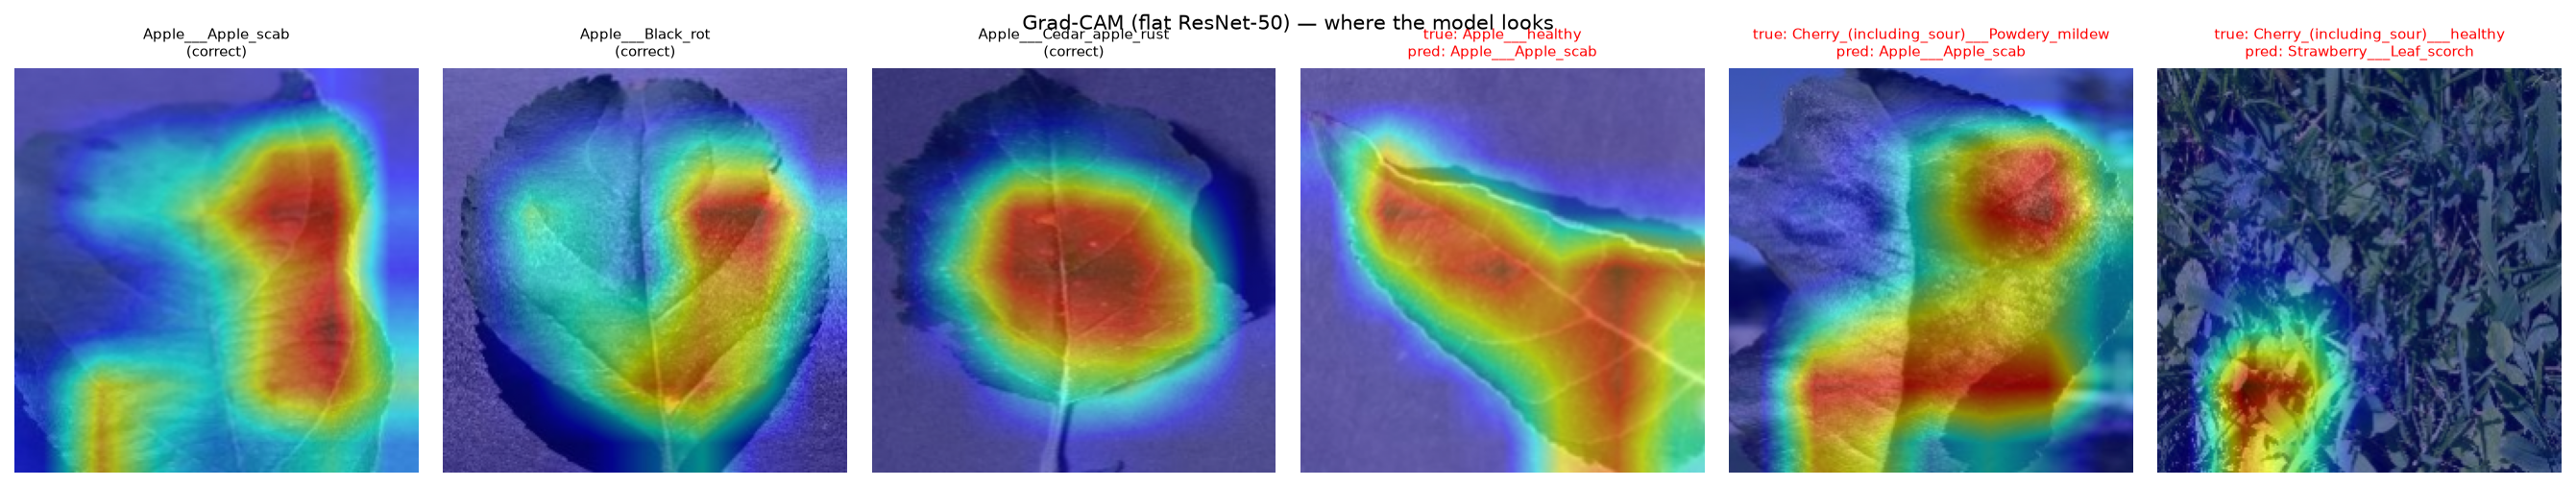
\includegraphics[width=\columnwidth]{gradcam.png}
  \caption{Grad-CAM mape ravnog modela: gde model ``gleda''. Toplota je pretežno
  na listu, ali difuzna.}
  \label{fig:gradcam}
\end{figure}

\subsection{Ograničenja}
Pored pristrasnosti na pozadinu, PlantVillage sadrži i \emph{približne duplikate}
(više snimaka istog lista), pa slučajna podela po slici može staviti slične
primere i u trening i u test, čime se metrike dodatno naduvavaju. Konačno, sve
metrike su merene na istom domenu (laboratorijske slike); validacija na
nezavisnom terenskom skupu ostaje za budući rad.

\subsection{Kada hijerarhija ipak ima smisla}
Iako ne donosi bolju tačnost, hijerarhija nudi \emph{interpretabilnost i
modularnost}: jasno se vidi da li greška nastaje na nivou vrste ili bolesti, a
pojedinačni klasifikatori se mogu nezavisno unapređivati (npr. ciljano za
najteže vrste --- krompir i kukuruz). To je kompromis između performanse i
interpretabilnosti.

\section{Zaključak}
Uporedili smo ravni i hijerarhijski pristup klasifikaciji biljnih bolesti na
PlantVillage skupu, uz evaluaciju prilagođenu neuravnoteženim podacima. Ravni
ResNet-50 postiže makro F1 od $0{,}9843$ naspram $0{,}9741$ za hijerarhiju, pa
hijerarhija \emph{ne donosi poboljšanje}; analiza propagacije greške pokazuje da
petina grešaka hijerarhije potiče od nivoa vrste. Najvažniji zaključak nije sama
visoka tačnost --- koja je očekivana i delom posledica svojstava skupa --- već
spoznaja da takve vrednosti precenjuju realnu upotrebljivost zbog pristrasnosti na
pozadinu. Budući rad obuhvata validaciju na terenskim slikama, grupisanje
približnih duplikata pri podeli, te ciljano unapređenje najtežih klasa.

\begin{thebibliography}{9}
\bibitem{mohanty2016} S. P. Mohanty, D. P. Hughes, and M. Salathé, ``Using deep
learning for image-based plant disease detection,'' \emph{Frontiers in Plant
Science}, vol. 7, 1419, 2016.
\bibitem{ferentinos2018} K. P. Ferentinos, ``Deep learning models for plant
disease detection and diagnosis,'' \emph{Computers and Electronics in
Agriculture}, vol. 145, pp. 311--318, 2018.
\bibitem{too2019} E. C. Too, L. Yujian, S. Njuki, and L. Yingchun, ``A
comparative study of fine-tuning deep learning models for plant disease
identification,'' \emph{Computers and Electronics in Agriculture}, vol. 161, pp.
272--279, 2019.
\bibitem{mohameth2020} F. Mohameth, C. Bingcai, and K. A. Sada, ``Plant disease
detection with deep learning and feature extraction using Plant Village,''
\emph{Journal of Computer and Communications}, vol. 8, no. 6, pp. 10--22, 2020.
\bibitem{noyan2022} M. A. Noyan, ``Uncovering bias in the PlantVillage dataset,''
\emph{arXiv preprint arXiv:2206.04374}, 2022.
\bibitem{gradcam2017} R. R. Selvaraju \emph{et al.}, ``Grad-CAM: Visual
explanations from deep networks via gradient-based localization,'' in
\emph{Proc. IEEE ICCV}, 2017, pp. 618--626.
\bibitem{focal2017} T.-Y. Lin, P. Goyal, R. Girshick, K. He, and P. Dollár,
``Focal loss for dense object detection,'' in \emph{Proc. IEEE ICCV}, 2017, pp.
2980--2988.
\bibitem{resnet2016} K. He, X. Zhang, S. Ren, and J. Sun, ``Deep residual
learning for image recognition,'' in \emph{Proc. IEEE CVPR}, 2016, pp. 770--778.
\bibitem{efficientnet2019} M. Tan and Q. V. Le, ``EfficientNet: Rethinking model
scaling for convolutional neural networks,'' in \emph{Proc. ICML}, 2019, pp.
6105--6114.
\end{thebibliography}

\end{document}
